\section{Phương pháp nghiên cứu}
\label{sec:methodology}

Hệ thống phát hiện vết dầu loang trên ảnh SAR được xây dựng dưới dạng quy trình tuần tự 2 giai đoạn (6 khối chức năng), chuyển đổi từ ảnh thô đơn kênh mức xám $I \in [0, 1]^{H \times W}$ sang mặt nạ nhị phân dự đoán $\hat{M} \in \{0, 1\}^{H \times W}$. Quá trình suy luận hoạt động độc lập hoàn toàn, không sử dụng bất kỳ nhãn tham chiếu ground truth nào. Sơ đồ kiến trúc tổng quan của hệ thống được minh họa trên Hình~\ref{fig:pipeline_overview}.

\begin{figure}[!t]
\centering
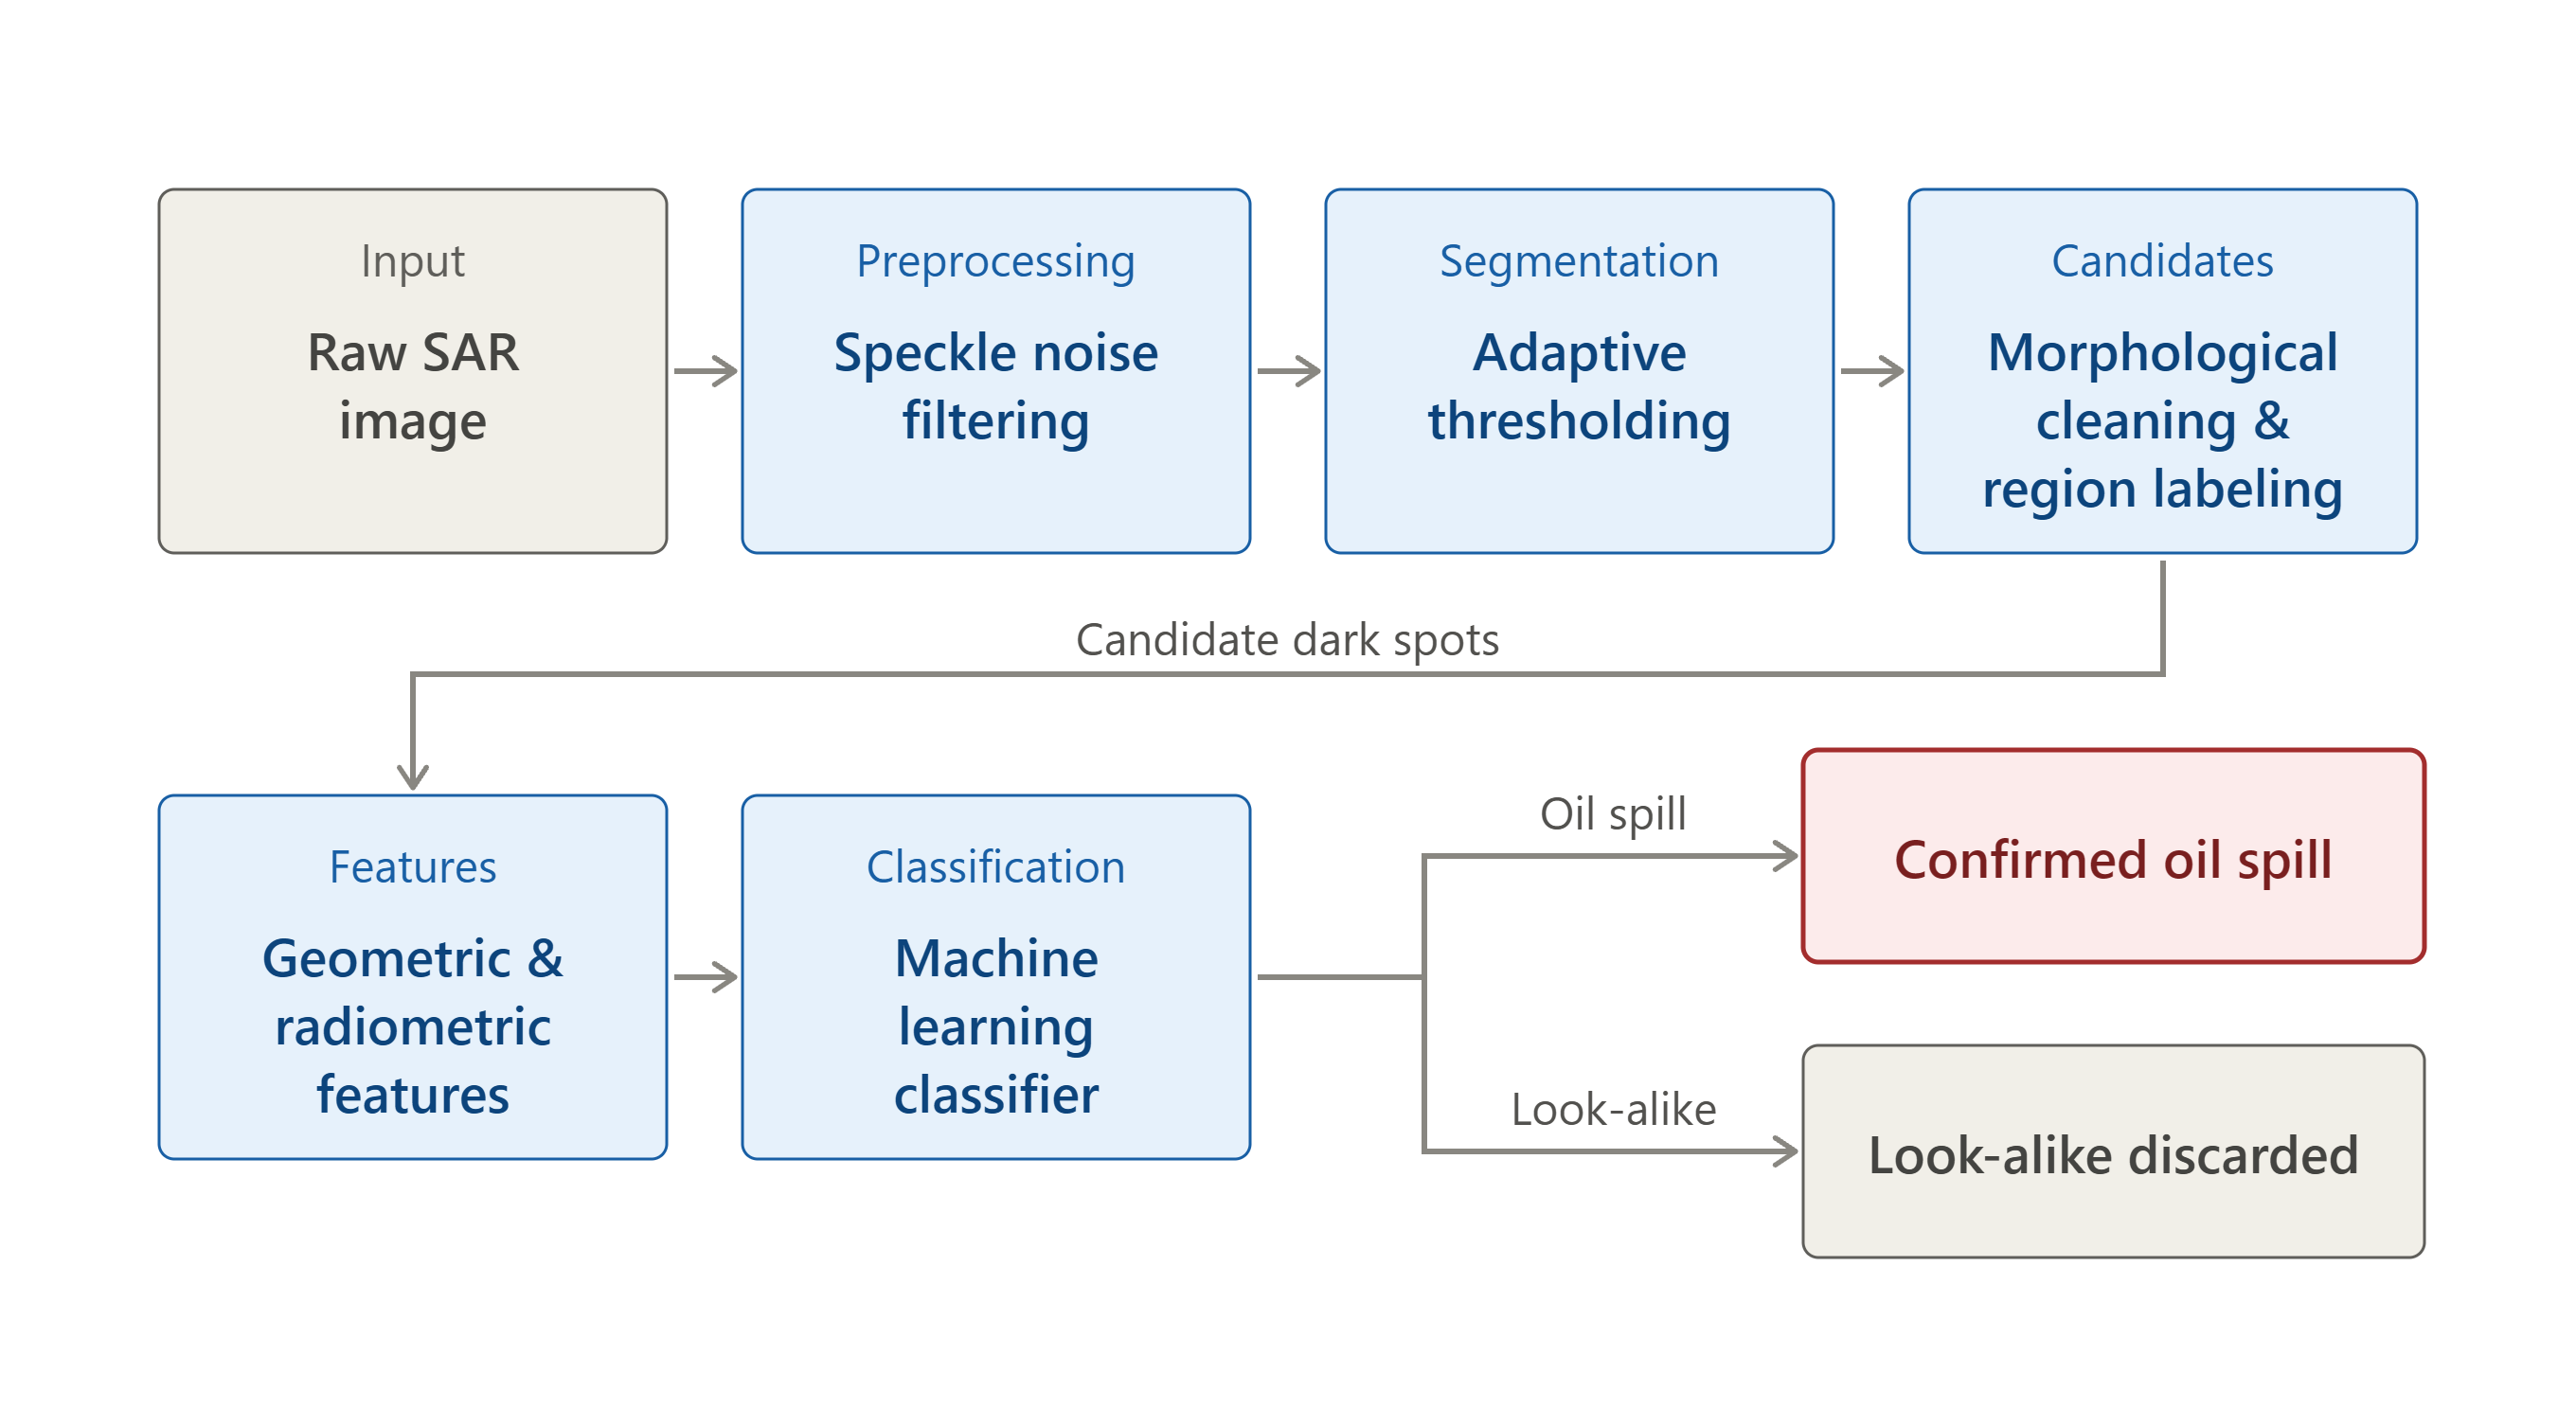
\includegraphics[width=0.95\linewidth]{figures/sar_oil_spill_detection_pipeline.png}
\caption{Sơ đồ khối kiến trúc tổng quan 2 giai đoạn của quy trình phát hiện vết dầu loang. Khối phân ngưỡng (\textit{Segmentation}) khảo sát ngưỡng tự động toàn cục Otsu $T^*$ (cấu hình chính) và ngưỡng thích nghi cục bộ Niblack; khối hậu xử lý thực hiện lọc diện tích $A_{\min} = 64$ pixels và gán nhãn liên thông 8 hướng; nhánh loại bỏ (\textit{Look-alike discarded}) trên bộ dữ liệu nhị phân SOS tương ứng với việc bác bỏ các vùng tối báo nhầm ($\hat{y}_i = 0$).}
\label{fig:pipeline_overview}
\end{figure}

\subsection{Khử nhiễu đốm bằng bộ lọc thống kê cục bộ Lee tối ưu hóa O(HW)}
\label{subsec:lee_filter}
Trên ảnh SAR cường độ tuyến tính thô, nhiễu đốm tuân theo mô hình thống kê nhân:
\begin{equation}
I(x, y) = R(x, y) \cdot u(x, y)
\end{equation}
trong đó $R(x, y)$ là hệ số phản xạ vô tuyến thực tế và $u(x, y)$ là thành phần nhiễu nhân có kỳ vọng $\mathbb{E}[u] = 1$, phương sai $\Var(u) = \sigma_u^2 = 1/L$ ($L$ là số looks tương đương của cảm biến).

Bộ lọc sai số toàn phương trung bình tối thiểu (Lee MMSE) xấp xỉ tuyến tính hóa hệ số phản xạ tại từng điểm ảnh thông qua trung bình cục bộ $m(x, y)$ và phương sai cục bộ $v(x, y)$:
\begin{equation}
\hat{R}(x, y) = m(x, y) + W(x, y) \cdot [I(x, y) - m(x, y)]
\label{eq:lee_formula}
\end{equation}
trong đó trọng số thích nghi $W(x, y) \in [0, 1]$ được xác định theo hệ số biến thiên cục bộ $C_I^2(x, y) = v(x, y) / m(x, y)^2$:
\begin{equation}
W(x, y) = \max\left(0, \frac{v(x, y) - \frac{m(x, y)^2}{L}}{\max(v(x, y), 10^{-12})}\right) = \max\left(0, 1 - \frac{1/L}{C_I^2(x, y)}\right)
\label{eq:lee_weight}
\end{equation}
Cấu hình chuẩn được khảo sát với kích thước cửa sổ $7 \times 7$, tham số $L \in \{1, 4\}$, và cơ chế đệm biên đối xứng (reflect padding). Cần lưu ý một đặc điểm quan trọng về miền giá trị dữ liệu: các ảnh trong bộ dữ liệu SOS được cung cấp dưới định dạng PNG 8-bit mức xám (chuẩn hóa tuyến tính về $[0, 1]$ bằng phép chia cho $255$) sau khi đã qua tiền xử lý khử đốm và nén dải động bởi nhà phát hành, chứ không còn ở miền công suất bức xạ $\sigma^0$ tuyến tính thuần túy. Do ảnh đã được làm trơn sơ bộ, số looks tương đương hiệu dụng thực tế trên các vùng biển đồng nhất ($\text{ENL}_{\text{eff}} = m^2 / v$) lớn hơn rất nhiều so với các giá trị danh định $L \in \{1, 4\}$. Hệ quả là điều kiện $C_I^2(x, y) \le 1/L$ (tức $v(x, y) \le m(x, y)^2/L$) xảy ra trên đại đa số điểm ảnh, làm cho trọng số $W(x, y) = 0$ và bộ lọc Lee với $L \le 4$ suy biến về bộ lọc trung bình hộp cục bộ $m(x, y)$.

\noindent\textbf{Tính toán mô-men cục bộ qua Bảng tổng tích lũy (Summed-Area Table):}
Ảnh mức xám được ép kiểu sang số thực độ chính xác kép 64-bit (\texttt{float64}) trên miền $[0, 1]$ nhằm tránh triệt tiêu số học. Chúng tôi xây dựng hai bảng tích phân hai chiều:
\begin{equation}
S(y, x) = \sum_{j \le y, i \le x} I(j, i), \quad S_2(y, x) = \sum_{j \le y, i \le x} I^2(j, i)
\end{equation}
Sau khi khởi tạo $S$ và $S_2$ với chi phí $\mathcal{O}(HW)$, giá trị trung bình $m(x, y)$ và trung bình bình phương $\mathbb{E}[I^2]$ trong bất kỳ cửa sổ hình chữ nhật kích thước $(2r+1) \times (2r+1)$ nào đều được tính toán trong thời gian $\mathcal{O}(1)$ thông qua 4 phép truy vấn góc:
\begin{equation}
\Sigma = S(y+r, x+r) - S(y-r-1, x+r) - S(y+r, x-r-1) + S(y-r-1, x-r-1)
\end{equation}
Phương sai cục bộ được tính có kẹp dưới không âm: $v(x, y) = \max(\mathbb{E}[I^2] - m(x, y)^2, 0)$. Nhờ đó, phép lọc thống kê cục bộ được hoàn tất với chi phí tính toán tuyến tính theo số điểm ảnh $\mathcal{O}(HW)$, hoàn toàn độc lập với bán kính cửa sổ lọc $r$.

\subsection{Phân đoạn tạo vùng ứng viên: Phân ngưỡng Otsu và Niblack}
\label{subsec:otsu_threshold}
Do hiện tượng làm phẳng sóng mao dẫn biển của vệt dầu, vùng dầu có cường độ tán xạ ngược thấp hơn nền biển. Thuật toán phân ngưỡng toàn cục Otsu chia biểu đồ mức xám (histogram) 256 bin của ảnh sau lọc $I_f$ thành hai lớp $\omega_0$ (vùng tối) và $\omega_1$ (nền biển) tại ngưỡng $t \in [0, 1]$ bằng cách tối đa hóa phương sai giữa hai lớp:
\begin{equation}
t^* = \arg\max_{t} \sigma_B^2(t), \quad \sigma_B^2(t) = \omega_0(t)\omega_1(t) [\mu_0(t) - \mu_1(t)]^2
\label{eq:otsu_between}
\end{equation}
trong đó $\omega_0(t), \omega_1(t)$ là xác suất tích lũy của hai lớp, và $\mu_0(t), \mu_1(t)$ là cường độ trung bình tương ứng. Mặt nạ nhị phân thô được xác định bởi:
\begin{equation}
B(x, y) = [I_f(x, y) < t^*]
\end{equation}
Đồng thời, tỷ số phương sai $\eta = \sigma_B^2(t^*) / \sigma_T^2 \in [0, 1]$ ($\sigma_T^2$ là tổng phương sai ảnh) được ghi nhận để chẩn đoán mức độ phân tách của histogram.

Đối với phân ngưỡng cục bộ Niblack trong cửa sổ trượt $W$, mặt nạ được xác định bởi:
\begin{equation}
B_{\text{Niblack}}(x, y) = [I_f(x, y) < m_W(x, y) - k \cdot s_W(x, y)]
\label{eq:niblack_formula}
\end{equation}
với $m_W, s_W$ là trung bình và độ lệch chuẩn cục bộ tính qua bảng tích lũy, và $k > 0$ là hệ số điều chỉnh (tương ứng với hệ số âm $-k$ trong ký hiệu chuẩn Niblack cho đối tượng tối trên nền sáng).

\subsection{Hậu xử lý diện tích và Gán nhãn liên thông 8 hướng}
\label{subsec:morphology_cca}
Để triệt tiêu các đốm nhiễu hạt nhỏ còn sót lại trên mặt biển mà không làm biến dạng biên vệt dầu, quy trình áp dụng ngưỡng diện tích thành phần liên thông tối thiểu $A_{\min} = 64$ pixels:
\begin{equation}
B_{\text{clean}} = \bigcup \{ \Omega_k \subset B \mid |\Omega_k| \ge A_{\min} \}
\end{equation}
Sau đó, mặt nạ nhị phân $B_{\text{clean}}$ được gán nhãn thành $K$ vùng ứng viên độc lập $\{\Omega_1, \Omega_2, \dots, \Omega_K\}$ bằng thuật toán Run-Length Union-Find 8 hướng với kỹ thuật nén đường đi (path compression).

\subsection{Không gian 8 đặc trưng vùng vật lý và xử lý ca biên}
\label{subsec:features}
Với mỗi vùng ứng viên $\Omega_i$ ($i = 1, \dots, K$), hệ thống trích xuất vector đặc trưng $\mathbf{x}_i = [f_0, f_1, \dots, f_7]^T \in \mathbb{R}^8$, bao gồm 4 đặc trưng hình học và 4 đặc trưng bức xạ/biên như được định nghĩa chi tiết trong Bảng~\ref{tab:features}.

\begin{table*}[!t]
\centering
\caption{Định nghĩa toán học và ý nghĩa vật lý của 8 đặc trưng vùng trích xuất cho mỗi thành phần liên thông $\Omega_i$.}
\label{tab:features}
\resizebox{\textwidth}{!}{%
\begin{tabular}{clclp{7.2cm}}
\toprule
\textbf{Ký hiệu} & \textbf{Tên đặc trưng} & \textbf{Nhóm} & \textbf{Công thức toán học} & \textbf{Ý nghĩa vật lý} \\
\midrule
$f_0$ & \texttt{area\_fraction} & Hình học & $A_i / (H \cdot W)$ & Tỷ lệ diện tích vùng so với diện tích toàn bộ khung ảnh viễn thám ($256 \times 256$ pixels). \\
$f_1$ & \texttt{elongation} & Hình học & $\sqrt{\frac{\lambda_2 + 10^{-6}}{\lambda_1 + 10^{-6}}}$ & Độ thuôn dài, tính từ hai trị riêng $\lambda_1 \le \lambda_2$ của ma trận hiệp phương sai tọa độ vùng. \\
$f_2$ & \texttt{extent} & Hình học & $A_i / (W_{\text{bbox}} \cdot H_{\text{bbox}})$ & Tỷ lệ lấp đầy của vùng so với diện tích hộp bao ngoài chữ nhật. \\
$f_3$ & \texttt{complexity} & Hình học & $P_i^2 / (4\pi A_i)$ & Độ phức tạp đường biên, với chu vi lưới $P_i$ đếm cạnh chuyển tiếp pixel. \\
\midrule
$f_4$ & \texttt{mean} & Bức xạ & $\mu_i = \frac{1}{A_i}\sum_{(x,y) \in \Omega_i} I_f(x, y)$ & Cường độ phản xạ SAR trung bình bên trong vùng ứng viên. \\
$f_5$ & \texttt{std} & Bức xạ & $\sigma_i = \sqrt{\frac{1}{A_i}\sum_{(x,y) \in \Omega_i} (I_f - \mu_i)^2}$ & Độ biến thiên cường độ mức xám nội vùng. \\
$f_6$ & \texttt{boundary\_gradient} & Biên & $\frac{1}{|\partial \Omega_i|}\sum_{(x,y) \in \partial \Omega_i} \|\nabla I_f(x, y)\|$ & Độ dốc biên trung bình: Sobel chuẩn hóa trên vành biên trong $\partial \Omega_i = \Omega_i \setminus (\Omega_i \ominus B_1)$. \\
$f_7$ & \texttt{background\_contrast} & Tương phản & $\frac{\mu_{\mathrm{bg}} - \mu_i}{|\mu_{\mathrm{bg}}| + 10^{-6}}$ & Độ tương phản bức xạ giữa vành đai nền biển 5 pixel ngoài biên và cường độ nội vùng. \\
\bottomrule
\end{tabular}%
}
\end{table*}

\noindent\textbf{Cơ chế xử lý ca biên, tính chất tự tham chiếu của nền và lý do loại trừ đặc trưng kết cấu:}
Khi trích xuất đặc trưng cho vùng $\Omega_i$:
\begin{enumerate}
    \item Hộp bao cục bộ được mở rộng thêm lề 5 pixel $[y_{\min}-5 : y_{\max}+6, x_{\min}-5 : x_{\max}+6]$ và kẹp chặt trong biên khung ảnh $[0, H) \times [0, W)$.
    \item Chu vi lưới $P_i$ và biên trong $\partial \Omega_i$ được tính toán trên mảng đệm ngoại vi bằng \texttt{False}, đảm bảo các cạnh tiếp giáp mép ảnh được tính chính xác vào chu vi và biên.
    \item Vành đai nền biển 5 pixel được xác định bởi $(\Omega_i \oplus B_5) \cap \{ \text{labels} == 0 \}$, chỉ lấy điểm ảnh ngoài vùng ứng viên. Cần lưu ý hai đặc tính cấu trúc của định nghĩa này: (a) Do tập hợp $\{\text{labels} == 0\}$ chủ yếu bao gồm các điểm ảnh có mức xám $\ge t^*$ (cùng một số đốm tối nhỏ $< A_{\min}$ vừa bị loại bỏ), giá trị $\mu_{\text{bg}}$ mang thiên lệch sáng có cấu trúc và phụ thuộc một phần vào chính ngưỡng Otsu $t^*$ (đặc trưng mang tính ``tự tham chiếu''); (b) Trong các khung cảnh ngập dầu diện rộng ($R_3/R_4$), khi ngưỡng Otsu buộc phải chia đôi chính mảng dầu đơn đỉnh hoặc khi vành đai 5 pixel rỗng khiến thuật toán chuyển sang nhánh dự phòng (fallback: tính $\mu_{\text{bg}}$ trên $I_f[\text{labels} == 0]$ hoặc trung bình toàn ảnh), tập $\{\text{labels} == 0\}$ thực chất lại là phần dầu sáng hơn. Khi đó, độ tương phản $f_7$ bị suy giảm mạnh một cách hệ thống, có thể khiến bộ phân loại bác bỏ nhầm vùng dầu thật.
    \item Khác với một số công trình kinh điển sử dụng ma trận đồng xuất hiện mức xám (GLCM)~\cite{brekke2005oil,singha2013oil}, nghiên cứu này không đưa nhóm đặc trưng kết cấu Haralick vào vector $\mathbf{x}_i$ vì hai lý do: (a) Ảnh PNG 8-bit trong bộ dữ liệu SOS đã qua làm mượt tiền xử lý khiến cấu trúc hạt vi mô bị triệt tiêu đáng kể, phần biến thiên mức xám nội vùng đã được đại diện bởi $f_5 = \sigma_i$; (b) Việc lượng tử hóa và tích lũy ma trận đồng xuất hiện 2 chiều theo nhiều hướng trên từng vùng liên thông có hình dạng bất kỳ làm tăng mạnh độ trễ khi một ảnh có hàng chục ứng viên.
\end{enumerate}

\subsection{Gán nhãn huấn luyện, Cân bằng lớp và Độ lệch với thước đo đánh giá}
\label{subsec:training_labels}
Trong giai đoạn huấn luyện, nhãn giám sát $y_i \in \{0, 1\}$ của từng vùng ứng viên được gán tự động dựa trên độ tinh khiết điểm ảnh (pixel purity) so với mặt nạ tham chiếu ground truth $G$:
\begin{equation}
\mathrm{Purity}(\Omega_i) = \frac{|\Omega_i \cap G|}{|\Omega_i|}
\end{equation}
Quy tắc gán nhãn phân tách:
\begin{itemize}
    \item \textbf{Vết dầu thật ($y_i = 1$):} $\mathrm{Purity}(\Omega_i) \ge 0.50$.
    \item \textbf{Vùng tối báo nhầm ($y_i = 0$):} $\mathrm{Purity}(\Omega_i) \le 0.05$.
    \item \textbf{Vùng biên trung gian ($0.05 < \mathrm{Purity} < 0.50$):} Loại bỏ khỏi tập huấn luyện để tránh nhiễu ranh giới quyết định.
\end{itemize}

Trên $2\,683$ ảnh huấn luyện Sentinel-1A, bước tạo ứng viên sinh ra tổng cộng $39\,530$ vùng ứng viên, gồm $11\,092$ vùng dương ($28.1\%$), $25\,946$ vùng âm ($65.6\%$) và $2\,492$ vùng trung gian ($6.3\%$). Để xử lý mất cân bằng lớp, chúng tôi áp dụng kỹ thuật lấy mẫu giảm ngẫu nhiên (undersampling) với seed cố định $2026$, chọn tối đa $10\,000$ mẫu mỗi lớp, tạo thành tập huấn luyện cân bằng gồm đúng $20\,000$ mẫu ($10\,000$ dương, $10\,000$ âm, tương ứng loại bỏ khoảng $61.5\%$ mẫu âm). Các đặc trưng được chuẩn hóa Z-score dựa trên kỳ vọng và độ lệch chuẩn $(\mu_k, \sigma_k)$ tính riêng trên tập huấn luyện:
\begin{equation}
z_{i,k} = \frac{x_{i,k} - \mu_k}{\max(\sigma_k, 10^{-12})}, \quad k = 0, \dots, 7
\end{equation}

\noindent\textbf{Sự khác biệt cấu trúc giữa nhãn huấn luyện (Purity) và thước đo đánh giá (Object IoU):}
Cần nhấn mạnh rằng $\mathrm{Purity}(\Omega_i) = |\Omega_i \cap G| / |\Omega_i|$ chuẩn hóa theo diện tích của riêng mảnh ứng viên $|\Omega_i|$, trong khi thước đo đánh giá cuối cùng ($\mathrm{IoU} = |\hat{\Omega}_p \cap G_q| / |\hat{\Omega}_p \cup G_q| \ge 0.50$) chuẩn hóa theo diện tích hợp với đối tượng tham chiếu nguyên khối $G_q$. Do đó, khi một vết dầu lớn $G_q$ bị bước phân ngưỡng Otsu cắt vụn thành nhiều mảnh nhỏ nằm trọn trong lòng vết dầu, mỗi mảnh đều có $\mathrm{Purity} = 1.0$ (nên bộ phân loại học cách giữ lại chúng như mẫu dương hợp lệ), nhưng từng mảnh riêng lẻ lại có $\mathrm{IoU} < 0.50$ so với $G_q$ (hoặc bị dư thừa do ràng buộc ghép cặp 1-1) và bị quy thành False Positive (FP) ở bước đánh giá đối tượng.

\subsection{Bộ phân loại LinearSVM với Tối ưu hóa Gradient Nesterov và CART}
\label{subsec:linearsvm}
Mô hình Linear Support Vector Machine tối ưu hóa hàm mục tiêu lồi có điều chuẩn $L_2$ trên toàn bộ vector trọng số $\mathbf{w} \in \mathbb{R}^9$ (gồm 8 trọng số đặc trưng và 1 hệ số chặn bias ở vị trí cuối) với hàm mất mát Squared-Hinge Loss:
\begin{equation}
\min_{\mathbf{w}} J(\mathbf{w}) = \frac{1}{2n}\|\mathbf{w}\|_2^2 + \frac{C}{n}\sum_{i=1}^n \max\left(0, 1 - y_i^* (\mathbf{z}_i^T \mathbf{w})\right)^2
\label{eq:svm_objective}
\end{equation}
trong đó $y_i^* = 2y_i - 1 \in \{-1, +1\}$, $\mathbf{z}_i = [z_{i,0}, \dots, z_{i,7}, 1]^T$, $n = 20\,000$ là số lượng mẫu huấn luyện, và $C = 10.0$ là siêu tham số phạt vi phạm lề.

Do hàm Squared-Hinge khả vi liên tục bậc một, gradient của $J(\mathbf{w})$ xác định bởi:
\begin{equation}
\nabla J(\mathbf{w}) = \frac{1}{n}\mathbf{w} - \frac{2C}{n}\sum_{i \in \mathcal{V}} y_i^* (1 - y_i^* \mathbf{z}_i^T \mathbf{w})\mathbf{z}_i
\end{equation}
với $\mathcal{V} = \{i \mid 1 - y_i^* \mathbf{z}_i^T \mathbf{w} > 0\}$ là tập các mẫu vi phạm lề. Bài toán được tối ưu hóa bằng thuật toán Nesterov Accelerated Gradient (NAG) với kỹ thuật tìm bước nhảy quay lui (backtracking line search) và tự động thiết lập lại xung lượng (adaptive restart). Điều kiện dừng hội tụ được áp dụng trên hàm mục tiêu đã chia trung bình cho $n = 20\,000$:
\begin{equation}
\|\nabla J(\mathbf{w})\|_\infty \le 10^{-6}
\end{equation}
(tương đương chuẩn vô cùng của gradient tổng chưa chia $n$ đạt $\approx 0.02$; tính hội tụ sát cực tiểu toàn cục được kiểm chứng trực tiếp đối chiếu với bộ giải chuẩn của \texttt{scikit-learn}, đạt độ lệch giá trị hàm mục tiêu $|J_{\text{NumPy}}^* - J_{\text{sklearn}}^*| = 2.88 \times 10^{-12}$ và đồng thuận dự đoán $100\%$). Vùng ứng viên $\Omega_i$ được phân loại là vết dầu loang tại ngưỡng quyết định cố định $\mathbf{z}_i^T \mathbf{w} > 0$.

Song song với LinearSVM, mô hình Cây quyết định CART được khảo sát làm mô hình đối sánh với tiêu chuẩn phân tách tạp chất Gini, độ sâu tối đa $\text{max\_depth} = 3$ và số mẫu tối thiểu tại nút lá $\text{min\_leaf} = 20$.
